\documentclass[conference, 10pt, letter]{IEEEtran}
\usepackage{verbatim}
\usepackage{multirow} \usepackage{enumerate}
\usepackage{amsmath,enumerate} \usepackage{amsthm}
\usepackage{algcompatible}
\usepackage{algpseudocode}
\usepackage{algorithm}
%\usepackage{algorithmic}
%\usepackage{pstricks}
\usepackage{amssymb, latexsym}
\usepackage{xfrac}
\usepackage{mathtools}
\usepackage{graphicx}
\usepackage[captionskip=5pt, nearskip=5pt, font=small]{subfig}
\DeclareGraphicsRule{*}{mps}{*}{}
\usepackage{listings}

%specific to this document only
%\usepackage{pgfplots}
\usepackage{pgfplotstable}
\pgfplotstableread{plts/experiment_erdren_edgecolor.tab}\erdrenone
\pgfplotstableread{plts/experiment_erdren_edgecolor_400.tab}\erdrentwo
\pgfplotstableread{plts/experiment_erdren_directededgecolor.tab}\erddirone
\pgfplotstableread{plts/experiment_erdren_directededgecolor_400.tab}\erddirtwo
\pgfplotstableread{plts/experiment_sclfre_edgecolor.tab}\sclfreeone
\pgfplotstableread{plts/experiment_sclfre_edgecolor_400.tab}\sclfreetwo
\pgfplotstableread{plts/experiment_smlwld_edgecolor.tab}\smlwldone
\pgfplotstableread{plts/experiment_smlwld_edgecolor_64.tab}\smlwldtwo
\pgfplotstableread{plts/experiment_smlwld_edgecolor_256.tab}\smlwldthree
\pgfplotstableread{plts/experiment8b1_av.tab}\averageone
\pgfplotstableread{plts/experiment8b2_av.tab}\averagetwo
\pgfplotstableread{plts/experiment8b3_av.tab}\averagethree
\pgfplotstableread{plts/experiment8b4_av.tab}\averagefour
\pgfplotstableread{plts/experiment_regular_16.tab}\regularone
\pgfplotstableread{plts/experiment_regular_32.tab}\regulartwo
\pgfplotstableread{plts/experiment_regular_64.tab}\regularthree
\pgfplotstableread{plts/experiment_regular_128.tab}\regularfour
%\pgfplotstableread{plts/experiment9a_av.tab}\stepping
%\pgfplotstableread{plts/experiment9a1_av.tab}\steppingone
%\pgfplotstableread{plts/experiment9a2_av.tab}\steppingtwo
%\pgfplotstableread{plts/experiment9a3_av.tab}\steppingthree
%\pgfplotstableread{plts/experiment9a4_av.tab}\steppingfour
%\pgfplotstableread{plts/experiment9b1_av.tab}\runningone
%\pgfplotstableread{plts/experiment9b2_av.tab}\runningtwo
%\pgfplotstableread{plts/experiment9b3_av.tab}\runningthree
%\pgfplotstableread{plts/experiment9b4_av.tab}\runningfour
%\pgfplotstableread{plts/experiment9b_av.tab}\running
%\pgfplotstableread{plts/experiment9c_av.tab}\costcomp
%\pgfplotstableread{plts/experiment9c1_av.tab}\costcompone
%\pgfplotstableread{plts/experiment9c2_av.tab}\costcomptwo
%\pgfplotstableread{plts/experiment9c3_av.tab}\costcompthree
\pgfplotstableread{plts/experiment8b1_rn.tab}\runsone
\pgfplotstableread{plts/experiment8b2_rn.tab}\runstwo
\pgfplotstableread{plts/experiment8b3_rn.tab}\runsthree
\pgfplotstableread{plts/experiment8b4_rn.tab}\runsfour
\pgfplotstableset{
  create on use/density/.style={
    create col/expr={\thisrow{nodes}+\thisrow{links}}}
    }
\pgfplotstableset{
  create on use/delta/.style={
    create col/expr={\thisrow{links}/\thisrow{nodes}}
    }}
\pgfplotstableset{
  create on use/nodebylinks/.style={
    create col/expr={(\thisrow{nodes}*\thisrow{links})}}
    }
\pgfplotscreateplotcyclelist{three}{% 
  every mark/.append style={fill=teal}\\% 
  every mark/.append style={fill=green}\\% 
  every mark/.append style={fill=orange}\\% 
}
\pgfplotscreateplotcyclelist{four}{%
  every mark/.append style={fill=teal}\\%
  every mark/.append style={fill=green}\\%
  every mark/.append style={fill=orange}\\%
  every mark/.append style={fill=pink}\\%
}
\pgfplotscreateplotcyclelist{three-1-0}{%
  every mark/.append style={fill=teal}\\% 
  every mark/.append style={fill=green}\\% 
  every mark/.append style={fill=orange}\\%
	every mark/.append style={fill=none}\\% 
	every mark/.append style={fill=none}\\% 
	every mark/.append style={fill=none}\\% 
}
\pgfplotscreateplotcyclelist{three-0-1}{%
	every mark/.append style={fill=none}\\% 
	every mark/.append style={fill=none}\\% 
	every mark/.append style={fill=none}\\% 
  every mark/.append style={fill=teal}\\% 
  every mark/.append style={fill=green}\\% 
  every mark/.append style={fill=orange}\\%
}
\pgfplotscreateplotcyclelist{four-1-0}{%
  every mark/.append style={fill=teal}\\%
  every mark/.append style={fill=green}\\%
  every mark/.append style={fill=orange}\\%
  every mark/.append style={fill=pink}\\%
	every mark/.append style={fill=none}\\%
	every mark/.append style={fill=none}\\%
	every mark/.append style={fill=none}\\%
	every mark/.append style={fill=none}\\%
}
\pgfplotscreateplotcyclelist{four-0-1}{%
	every mark/.append style={fill=none}\\%
	every mark/.append style={fill=none}\\%
	every mark/.append style={fill=none}\\%
	every mark/.append style={fill=none}\\%
  every mark/.append style={fill=teal}\\%
  every mark/.append style={fill=green}\\%
  every mark/.append style={fill=orange}\\%
  every mark/.append style={fill=pink}\\%
}

%%%%%%%%%%%%%

\usepackage{pgf}
\usepackage{tikz}
\usetikzlibrary{decorations.pathmorphing} % LATEX and plain TEX when using Tik Z
\usetikzlibrary{positioning}
\usetikzlibrary{er}
\usetikzlibrary{automata}
\usetikzlibrary{shapes.geometric}
\usetikzlibrary{shapes.misc}
\tikzstyle{vx}=[draw,circle,fill=white,minimum size=2pt, inner sep=1pt, node distance=15mm]
\tikzstyle{ex}=[draw,rectangle,fill=white,minimum size=2pt, inner sep=3pt, node distance=15mm]
\tikzstyle{nfo}=[anchor=north west, rectangle, fill=white,text width=4cm, inner sep=3pt, node distance=15mm]
\tikzstyle{bup}=[semithick, decoration={bent, aspect=.3, amplitude=4}, decorate, ->, >=stealth]
\tikzstyle{bdn}=[semithick, decoration={bent, aspect=.3, amplitude=-4}, decorate, ->, >=stealth]
\tikzstyle{BUP}=[thick, decoration={bent, aspect=.3, amplitude=8}, decorate, ->, >=stealth]
\tikzstyle{BDN}=[thick, decoration={bent, aspect=.3, amplitude=-8}, decorate, ->, >=stealth]
\tikzstyle{MUP}=[thick, decoration={bent, aspect=.3, amplitude=16}, decorate, ->, >=stealth]
\tikzstyle{MDN}=[thick, decoration={bent, aspect=.3, amplitude=-16}, decorate, ->, >=stealth]
\tikzstyle{pln}=[draw, dotted]
\tikzstyle{dir}=[draw, dotted, decorate, ->, >=stealth, bend left=10]
\tikzstyle{str}=[semithick, decorate, ->, >=stealth]
\tikzstyle{cr}=[draw, circle, fill=black!25,minimum size=150pt]
\tikzstyle{rst}=[state, shape=rounded rectangle, rounded rectangle arc length=90, text width=2cm, inner sep=4pt]
\tikzstyle{rsf}=[state, fill=green!35, shape=rounded rectangle, rounded rectangle arc length=90, text width=1.75cm, inner sep=4pt]
%styles for plots?
\tikzstyle{bls}=[blue, solid, mark=square*]
\tikzstyle{grt}=[red, solid, mark=*]
\tikzstyle{inv}=[draw=none]

% \paperheight=11in \paperwidth=8.5in \textheight=9.0in
% \textwidth=6.5in \voffset=-.875in \hoffset=-.875in
\newenvironment{code} {\begin {quote}\begin{footnotesize}}
    {\end{footnotesize}\end{quote}}

% \oddsidemargin 0.0 in \evensidemargin 0.0 in
\newenvironment{enumeratealpha}
{\begin{enumerate}[(a{\textup{)}}]}{\end{enumerate}}

\theoremstyle{plain}
\newtheorem{lem-rule}{Rule}
\newtheorem{thm}{Theorem}
\newtheorem{con}{Conjecture}
\newtheorem{lem}{Lemma}[thm]
\newtheorem{prp}{Proposition}
\newtheorem{prop}{Proposition}[con]
\newtheorem{lprp}{Proposition}[lem]
\newtheorem{cor}{Corollary}[lem]
\theoremstyle{definition}
\newtheorem{defn}{Definition}[thm]
\newtheorem{defi}{Definition}
\newtheorem{dfn}{Definitions}[thm]
\newtheorem{ldef}{Definition}[lem]
\newtheorem{assm}{Assumption}
\theoremstyle{remark}
\newtheorem*{smy}{Summary}
\newtheorem{note}{Note}[thm]
\newtheorem{case}{Case}
%algorithms commands
\algblockdefx[Case]{Case}{EndCase} %
[1] [{\em var}] {{\bfseries case} {\em #1\ } } %
{{\bfseries end case}}%
\algcblockdefx[Case]{Case}{When}{EndCase}
[1] [{\em true}] {{\bfseries when} {\em #1\ }}
{{\bfseries end case}} %

\algblockdefx[TimesDo] {DoTimes}{EndTimes}
[1] [0] {#1 times {\bfseries do}}
{{\bfseries end do}}

%subalgorithms environment
\makeatletter
\newcounter{parentalgorithm}
\newenvironment{subalgorithms}{%
%  \refstepcounter{algorithm}%
  \floatname{algorithm}{Procedure}
  \protected@edef\theparentalgorithm{\thealgorithm}%
  \setcounter{parentalgorithm}{\value{algorithm}}%
  \setcounter{algorithm}{0}%
  \def\thealgorithm{\theparentalgorithm-\alph{algorithm}}%
  \ignorespaces
}{%
  \setcounter{algorithm}{\value{parentalgorithm}}%
  \ignorespacesafterend
}
\makeatother

%code environments
\usepackage{float}
 
\floatstyle{ruled}
\newfloat{codeblock}{thp}{lop}
\floatname{codeblock}{Example}

\lstnewenvironment{rubyblock} 
{\lstset{language=Ruby, breaklines=true, basicstyle=\small, xleftmargin=10pt, numbers=left, numberstyle=\tiny, stepnumber=1, numbersep=5pt, escapeinside={|;}{;|}}}
{}
% text macros
\def\cI{{\mathcal I}} \def\cR{{\mathcal R}} \def\cE{{\mathcal E}}
\def\cC{{\mathcal C}} \def\cF{{\mathcal F}} \def\cU{{\mathcal U}}
\def\cH{{\mathcal H}} \def\cD{{\mathcal D}} \def\cB{{\mathcal B}}
\def\cQ{{\mathcal Q}} \def\cV{{\mathcal V}} \def\cS{{\mathcal S}}
\def\cG{{\mathcal G}} \def\cA{{\mathcal A}} \def\cO{{\mathcal O}}
\def\cW{{\mathcal W}} \def\cL{{\mathcal L}} 

\def\bI{{\mathbb I}} \def\bO{{\mathbb O}}
\def\bC{{\mathbb C}} \def\bM{{\mathbb M}}
\def\bId{{$\mathbb I$}} \def\bOd{{$\mathbb O$}}
\def\bCd{{$\mathbb C$}} \def\bMd{{$\mathbb M$}}

\def\cId{{$\mathcal I$}} \def\cRd{{$\mathcal R$}} \def\cEd{{$\mathcal E$}} 
\def\cCd{{$\mathcal C$}} \def\cFd{{$\mathcal F$}} \def\cUd{{$\mathcal U$}} 
\def\cHd{{$\mathcal H$}} \def\cDd{{$\mathcal D$}} \def\cBd{{$\mathcal B$}} 
\def\cQd{{$\mathcal Q$}} \def\cVd{{$\mathcal V$}} \def\cSd{{$\mathcal S$}} 
\def\cGd{{$\mathcal G$}} \def\cAd{{$\mathcal A$}} \def\cOd{{$\mathcal O$}}
\def\cWd{{$\mathcal W$}} \def\cLd{{$\mathcal L$}}

\def\suchthat{{\: |\:}}




\bibliographystyle{IEEEtranS}

\begin{document}
\title{Two Edge Coloring Algorithms Using a Simple Matching Discovery Automata}

\author{\IEEEauthorblockN{J. Paul Daigle and Sushil K. Prasad}
\IEEEauthorblockA{Department of Computer Science\\
Georgia State University\\
Atlanta, Georgia 30303, USA\\}
}

\maketitle

\begin{abstract}
We here present two probabilistic edge coloring algorithms for a message passing model of distributed computing. The algorithms use a simple automata for finding a matching on a graph to produce the colorings. Our first algorithm for edge coloring finds an edge coloring of a graph which is guaranteed to use no more than $2\Delta - 1$ colors and completes in $O(\Delta)$ communication rounds using only one hop information, where $\Delta$ is the greatest degree of the graph. Our second algorithm finds a strong edge coloring of a symmetric digraph in $O(\Delta)$ communication rounds, using only one hop information. 
\end{abstract}

\section{Introduction}
In this paper, we use the matching based automata used in \cite{Daigle:2011uq} and shown in Figure~\ref{fig:automata} as the basis for two different edge-coloring algorithms, edge coloring of an undirected graph and strong edge coloring of a directed graph. A practical distributed algorithm for the last problem is of some interest in networking, as it can be used as a model for channel or time-slot assignment in an adhoc network \cite{1598948, 1498534}.

Our algorithms are probabilistic and compete well with other probabilistic algorithms. For the edge coloring problem, our algorithm produces a coloring which is no greater than $2\Delta - 1$ in $O(\Delta)$ rounds in the typical case, where $\Delta$ is the maximum degree of the graph. Our algorithm for strong directed coloring produces a correct coloring in $O(\Delta)$ rounds. 

\begin{figure}[htp]
  \begin{center}
  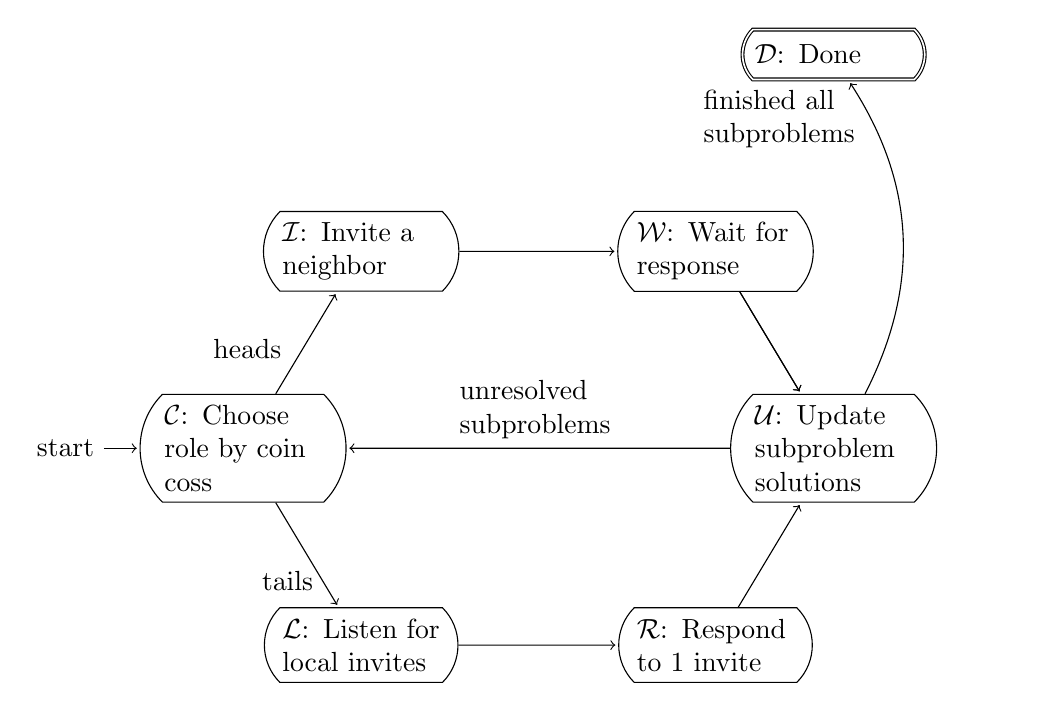
\begin{tikzpicture}[shorten >=1pt,node distance=1cm,on grid,auto, bend angle=75, every state/.style={scale=1, minimum size=18pt, inner sep=2pt}]
    %\draw [help lines] (-5,-4) grid (7,4);
    \path [help lines] (-4,-4) grid (7,4);
		
    \node [rst, initial]   (C) at (-3,-1) {\cCd: Choose role by coin coss};
    \node [rst] (I)            at (-1.5,1.5) {\cId: Invite a neighbor};
    \node [rst] (L)            at (-1.5,-3.5) {\cLd: Listen for local invites};
    \node [rst] (W)            at (3,1.5)  {\cWd: Wait for response};
    \node [rst] (R)            at (3,-3.5) {\cRd: Respond to 1 invite};
    \node [rst] (U)            at (4.5,-1) {\cUd: Update subproblem solutions};
    \node [rst, accepting] (D) at (4.5,4)  {\cDd: Done};

    \path [->] (C) edge              node [near start] {heads} (I)
               (C) edge              node [near end, left] {tails} (L)
               (L) edge              node {} (R)
               (I) edge              node {} (W)
               (W) edge              node {} (U)
               (R) edge              node {} (U);
    \path [->] (U) edge [bend right=30]             node [very near end, left, text width=2cm] {finished all subproblems} (D);
    \path [->] (W) edge  node {} (U);
    \path [->] (U) edge  node [above, text width=2cm] {unresolved subproblems} (C);

  \end{tikzpicture}
  \caption{Distributed Matching and Computation Automata}
  \label{fig:automata}
  \end{center}
\end{figure}
 
Our algorithms assume a message based model of computing, so we can assume that compute nodes are synchronized and that each node can communicate with each of its neighbors in each round \cite{1146387}. Each node is therefore assumed to move synchronously through each stage of the algorithm. 

Our main contribution is extending the framework developed in \cite{Daigle:2011uq} to a new set of problems. The algorithms based on the framework are competitive with know algorithms in time complexity and provide high quality solutions. We believe that this basic approach can be modified and extended to solve a variety of problems, providing a simple starting point for the development of new distributed, probabilistic algorithms that provide constant approximations for NP complete problems.

\subsection{Problem Definitions}
\input{secs/sec-definitions.tex}
\subsection{Prior Work}
Distributed edge coloring is a well studied problem. Panconesi and collaborators have produced a number of papers tying edge coloring to channel assignment and presenting novel edge coloring algorithms with communication complexity of as low as $O(log{log{n}})$ \cite{Grable:1997:NOD:314161.314266},\cite{Panconesi:1997:RDE:249364.249368},\cite{1041515},\cite{982945}.

Gandham et al. present an deterministic algorithm which colors a graph using $\Delta + 1$ colors with a time complexity of $2\Delta + 1$ for acyclic graphs \cite{1498534}. Barenboim et al. present a deterministic algorithm which extends beyond trees and provides an $O(\Delta)$ coloring in $O(\Delta^{1 + \epsilon)}$ time for an arbitrarily small constant $\epsilon \le 1$ \cite{Barenboim:2011:DDE:1993806.1993825}. A limitation of this algorithm is that the constant factor for quality increases as $\epsilon$ decreases.

In strong edge coloring, Barret et al. present algorithms with running times dependent on the size of the graph $n$ \cite{1598948}. Kanj et al. show tight bounds for the quality and locality, but not the time bounds, of their algorithms \cite{Kanj:2009:LAE:1696884.1696902}.

\subsection{The Message Passing Model}
\input{secs/sub-message-passing-caveats.tex}

\section{Edge Color Algorithm}
\subsection{Algorithm}
\input{secs/sub-edge-description.tex}
\begin{algorithm}
\caption{Distributed Matching Based Edge-Coloring Algorithm}
\begin{algorithmic}[1]
%\Require {$G(V,E)$: a Communicaton Network}
\ForAll {$v_u \in V$ in parrallel}
\State {$live_u \gets C$} \Comment All colors are available \label{alglin:ec-init-color}
\State {$dead_u \gets \{\}$} \Comment No colors are used \label{alglin:ec-init-dict}
\State {$used_u \gets [\,]$} \Comment No colors are assigned
\State state $\leftarrow$ \cCd
\Repeat
\If {state = \cCd}
\State {State $\gets (\cI \lor \cL)$} \Comment Coin toss selects state

\ElsIf {state = \cId}
\State {Randomly select an uncolored edge, $e_{u,v}$}\label{alglin:ec-issue-invite}
\State {$c \gets (live_u \smallsetminus used_v[1]$} \Comment assign first available color to $c$ \label{alglin:ec-select-color}
\State {Broadcast $I_u^v,c$} \Comment $u$ Invites $v$ to color $e_{u,v} \text{ with } c$ 
\State {state $\leftarrow$ \cWd}

\ElsIf {state = \cLd}
\State {Recieve $I_x^y,c$} \Comment all local invites
\If {$y = u$} \Comment invite is targeted to $v_u$
\State {store $I_x^y,c$}
\EndIf
\State {State $\gets \cR$}

\ElsIf {state = \cRd}
\State {Randomly Select $I_v^u,c$} \Comment from stored invites \label{alglin:ec-choose-invite}
\State {Broadcast $R_u^v,c $} \Comment $u$ accepts $v's$ invitation
\State {Assign $c \mapsto e_{u,v}$} 
\State {$used_u \hookleftarrow c$} \Comment Append c to assigned colors \label{alglin:ec-assign1}
\State {state $\gets \cU$}

\ElsIf {state = \cWd}\label{alglin:ec-receive-responses}
\State {Recieve $R_x^y,c$} \Comment all local responses
\If {$y = u$} \Comment response is to $v_u$ 
\State {Assign $c \mapsto e_{u,v}$} 
\State {$used \hookleftarrow c$} 
\EndIf
\State {state $\gets \cU$}

\ElsIf {state = \cUd}
\State {Broadcast $used_u$} \Comment Broadcast all assigned edge colors
\State {Recieve $used_v$} \Comment Receive neighbors assigned colors
\State {$dead_u \hookleftarrow used_v$}  \Comment the "dead" set contains the used colors from each neighbor, and is used when choosing colors in the invitation step \label{alglin:ec-assign2}
\State {state $\gets \cE$}

\ElsIf {State = \cEd}
\State {Subtract $used_u$ from $live_u$} \Comment update usable colors \label{alglin:ec-update-colors}
\State {state $\gets \cC$}

\EndIf
\Until {All edges are assigned a color}\label{alglin:ec-end-while}
\EndFor
\end{algorithmic}
\label{alg:edge-color}
\end{algorithm}



\subsection{Algorithm Analysis}

We here address the termination, correctness, and solution quality of Algorithm~\ref{alg:edge-color}. We will first show that Algorithm~\ref{alg:edge-color} is likely to terminate in $O(\Delta)$ rounds, then that it will produce a correct coloring if it does terminate, and finally that the coloring produced will use no more than $2\Delta - 1$ colors.
\begin{lemm}
\label{lem:edge-color-terminate}
Algorithm~\ref{alg:edge-color} is likely to terminate in $O(\Delta)$ rounds.
\end{lemm}

\begin{lemm}
\label{lem:edge-color-correct}
Algorithm~\ref{alg:edge-color} produces a correct coloring. 
\end{lemm}

\begin{lemm}
\label{lem:edge-color-approximate}
Algorithm~\ref{alg:edge-color} will use $2\Delta - 1$ colors in the worst case. 
\end{lemm}

\begin{proof}
We first show that Algorith~\ref{alg:edge-color} terminates in $O(\Delta)$ rounds.

\begin{lemm}
\label{lem:edge-color-terminate}
Algorithm~\ref{alg:edge-color} is likely to terminate in $O(\Delta)$ rounds.
\end{lemm}

We will now show that the coloring produced by Algorithm~\ref{alg:edge-color} is guaranteed to be correct.
\begin{lemm}
\label{lem:edge-color-correct}
Algorithm~\ref{alg:edge-color} produces a correct coloring. 
\end{lemm}

We now show that the coloring produced by Algorithm~\ref{alg:edge-color} can be no worse than $2\Delta - 1$ in the worst case.
\begin{lemm}
\label{lem:edge-color-approximate}
Algorithm~\ref{alg:edge-color} will use $2\Delta - 1$ colors in the worst case. 
\end{lemm}

Therefore, Theorem~\ref{thm:edge-color} is correct.
\end{proof}

\begin{con}
\label{lem:edge-color-optimal}
Algorithm~\ref{alg:edge-color} uses $C \le \Delta + 1$ colors in the typical run. 
\end{con}

\begin{proof}[Discussion of Conjecture~\ref{lem:edge-color-optimal}]

A graph can certainly be colored with either $\Delta$ or $\Delta + 1$ colors. If a node $v$ were to be forced to use $\Delta + 2$ colors to color a graph, that would mean that there are two colors of index $\le \Delta$ which are being used by each neighbor of $v$ but not by $v$ itself.

In order for this to happen, there would need to be some round, or sequentially set of rounds, in which all of $v$'s neighbors formed a matching, and $v$ did not. We know from Proposition~\ref{lem:edge-color-terminate} that the odds of a node forming a match in a given round are greater than $\sfrac{1}{4}$, because the odds of a node being an invitor and recieving an invitation are approximately $\sfrac{1}{4}$. We can also easily calculate that the odds of a node being an invitor and sending a successful invitation are no greater than $\sfrac{1}{4}$, since there is a $\sfrac{1}{2}$ chance that a node $w$ will choose to send invitations and a $\sfrac{1}{2}$ chance that the neighbor $w$ sends an invitation to is an invitee.  

So the odds of a node forming a pair at all in a given round are $\sfrac{1}{x}$, $4 \ge x \ge 2$. 

For a given node to not form a pair while all of its neighbors do form pairs is therefore akin to the odds that in a fair coin toss, we first flip heads and then flip tails some arbitrary number of times in a row, or that in a simultaneous coin toss of some number of coins, one is heads while the rest are tails. 

We therefore expect our algorithm to behave well in the following sense: we should get conistent results with similar graphs, the algorithm should color with $\Delta$ or $\Delta + 1$ colors most of the time, and in no experimental case should we ever see the maximum $2\Delta - 1$ colors used.

\end{proof}


\section{DiMa2ed Algorithm}
\subsection{Algorithm}
\label{sub:dima2ed-description}
\input{algs/alg-ma2ed.tex}
\input{secs/sub-dima2ed-description.tex}
\subsection{Algorithm Analysis}
We here address the termination and correctness of Algorithm~\ref{alg:ma2ed}.
\input{prfs/pro-ma2ed.tex}
\section{Experiments and Results}
\subsection{Algorithm~\ref{alg:edge-color}  on Erdos-Renyi Graphs}
\input{secs/sub-experiment-erdren.tex}
\subsection{Algorithm~\ref{alg:edge-color} on Scale-Free Graphs}
\label{sub:experiment:scalefree}
\input{secs/sub-experiment-scalefree.tex}
\subsection{Algorith~\ref{alg:edge-color} on Small World Graphs}
\input{secs/sub-experiment-smallworld.tex}
\subsection{Algorithm~\ref{alg:ma2ed} on Erdos-Renyi Graphs}
\label{sub:experiment-erdren-direct}
\input{secs/sub-experiment-erdren-direct.tex}
\section{Conclusion}
\input{secs/sec-conclusion.tex}

\bibliography{edge-color}

\end{document}
